\section{Profiling Results} \label{sec:profiling}

We produce the profiling results from our source code, and we release our source code on GitHub.\footnote{https://github.com/calzonelover/Profiling-Transformer-Based-Model}

\subsection{RoBERTa}

\subsubsection{Configurations}
The configurations for RoBERTa model are as follows:
\begin{itemize}
    \item Batch size: 8
    \item GPU: 1, 2 and 4
    \item Model name: Wangchanberta (Thai RoBERTa model) \cite{wangchanberta2021}
    \item Dataset: Wongnai\_reviews (Text classification)
    \item Epoch: 1
\end{itemize}

\subsubsection{Results}
The simplest way to observe longest running interface could be done by aggregating each running interface. According to the Table~\ref{fig:bert:tg}, top 10 interfaces in single and double GPUs are all matrix multiplicative operations. On the other hand, most of  top 10 interfaces in 4 GPUs are collective communication in the GPU devices which are reduce and broadcast interfaces to transfer the data around the system. This is the first obvious clue to perform further study about how they spend the time on each group of interface to determine the problem from low level aspect.

\begin{figure}[htbp]
    \centering
    \begin{subfigure}{.5\textwidth}
        \centering
        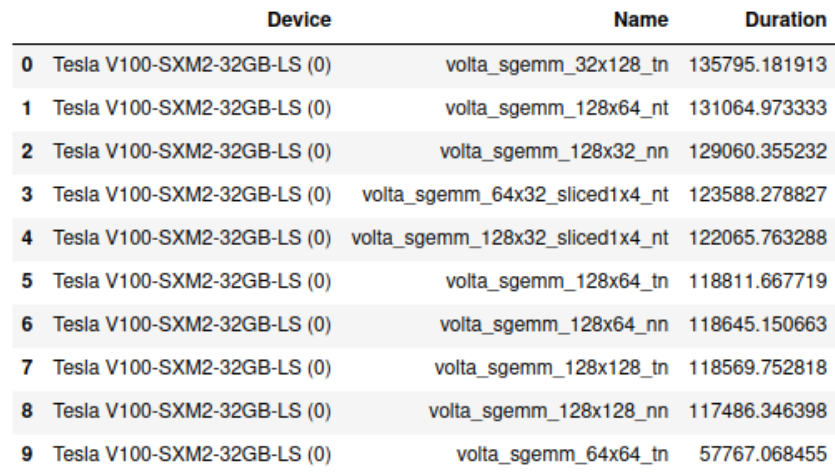
\includegraphics[width=\linewidth]{fig/bert/bert_t1.png}
        \caption{1 GPUs}
        \label{fig:bert:timegroup}
    \end{subfigure}%
    \begin{subfigure}{.5\textwidth}
        \centering
        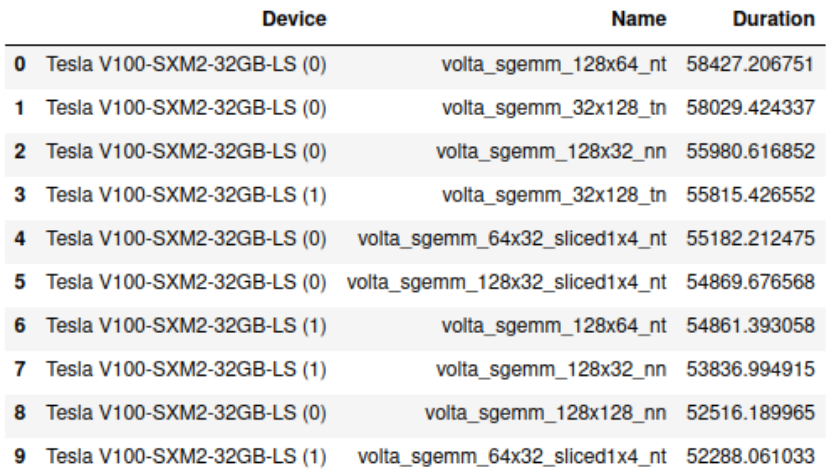
\includegraphics[width=\linewidth]{fig/bert/bert_t2.png}
        \caption{2 GPUs}
        \label{fig:bert:timegroup_frac}
    \end{subfigure}
    \begin{subfigure}{.6\textwidth}
        \centering
        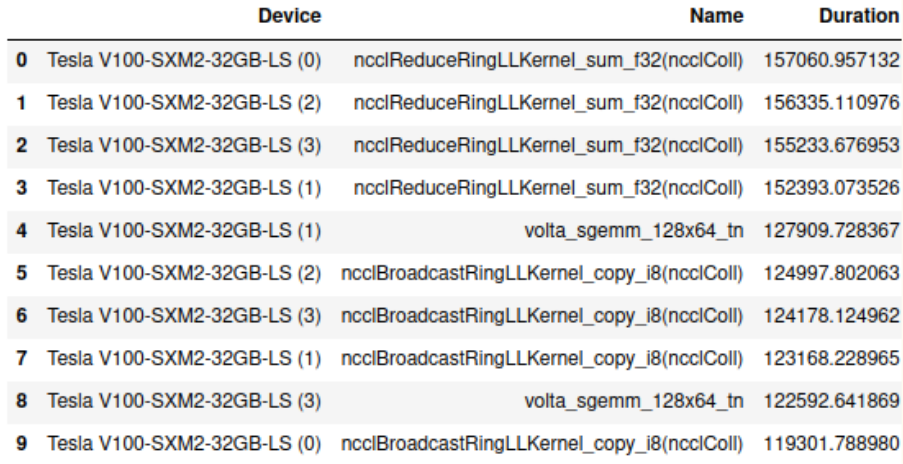
\includegraphics[width=\linewidth]{fig/bert/bert_t4.png}
        \caption{4 GPUs}
        \label{fig:bert:timegroup_frac}
    \end{subfigure}    
    \caption{Top 10 longest running interfaces}
\label{fig:bert:tg}
\end{figure}


The big picture of the problem can be seen by visualizing the aggregated running time of each operation group as in Figure~\ref{fig:bert:group_runtime}. It can bee seen that increasing the number of GPU will increase the spending time in memory management operations which is what we suspect in the first place. Moreover, running this model on four GPUs does induce a lot of collective communication across the devices to send the data back and forth. The memory management operation is more than 30\% of the overall running time. This is very critical for the scalability. It also implicitly means that the speed up factor after adding more than 4 GPUs might not significant anymore. Hence, we probably under-utilize the resource when training BERT model with more than four GPUs.


\begin{figure}[htbp]
    \centering
    \begin{subfigure}{.5\textwidth}
        \centering
        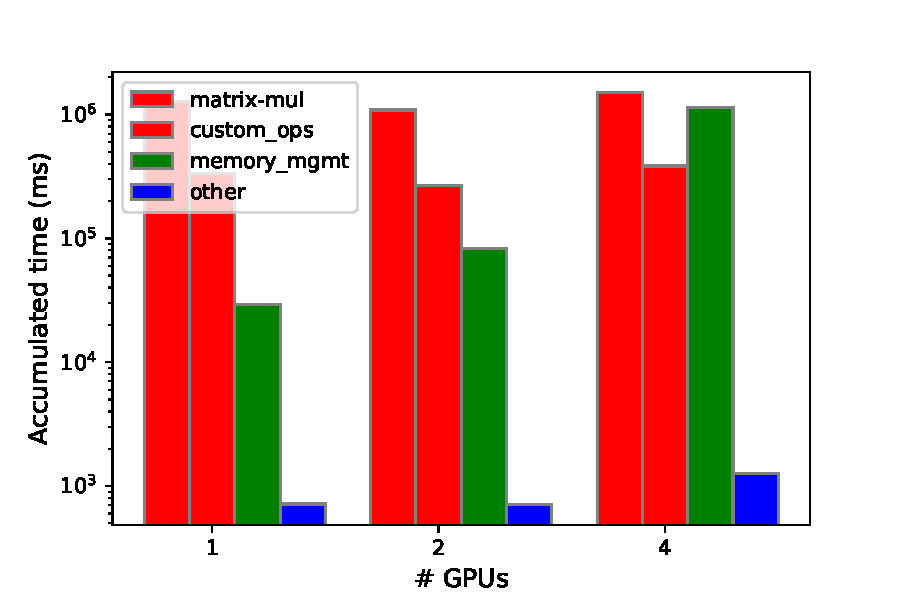
\includegraphics[width=\linewidth]{fig/bert/timegroup.pdf}
        \caption{Real spending time}
        \label{fig:bert:timegroup}
    \end{subfigure}%
    \begin{subfigure}{.5\textwidth}
        \centering
        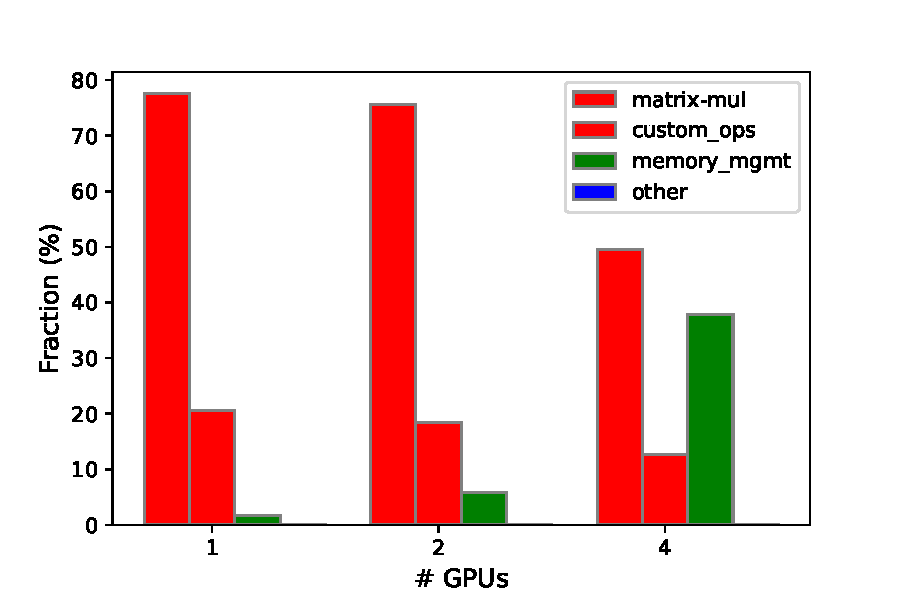
\includegraphics[width=\linewidth]{fig/bert/timegroup_frac.pdf}
        \caption{Fraction of time}
        \label{fig:bert:timegroup_frac}
    \end{subfigure}
    \caption{Spending time of multiple group of operations}
\label{fig:bert:group_runtime}
\end{figure}

\begin{figure}[htbp]
    \centering
    \begin{subfigure}{.5\textwidth}
      \centering
      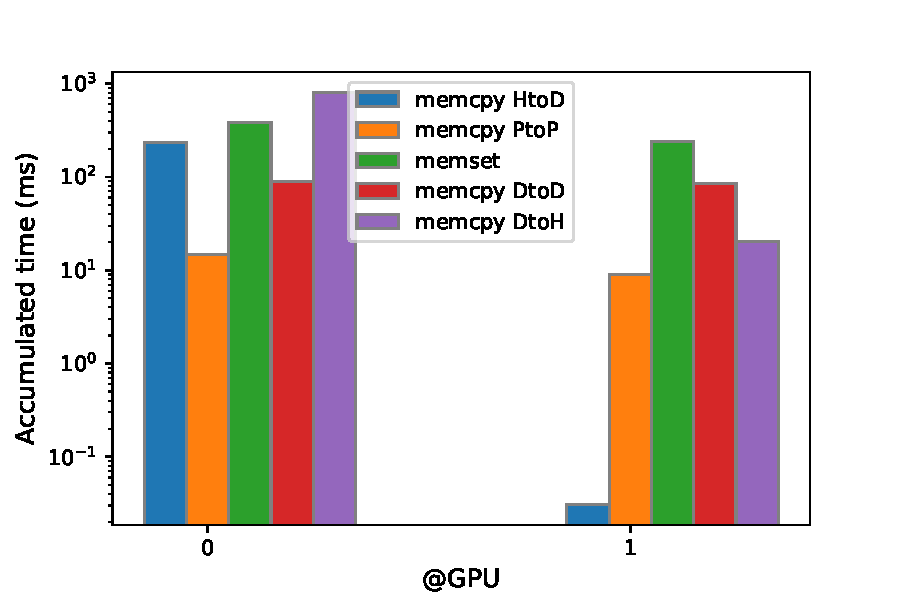
\includegraphics[width=\linewidth]{fig/bert/mem_2gpus.pdf}
      \caption{2 GPUs}
    \end{subfigure}%
    \begin{subfigure}{.5\textwidth}
      \centering
      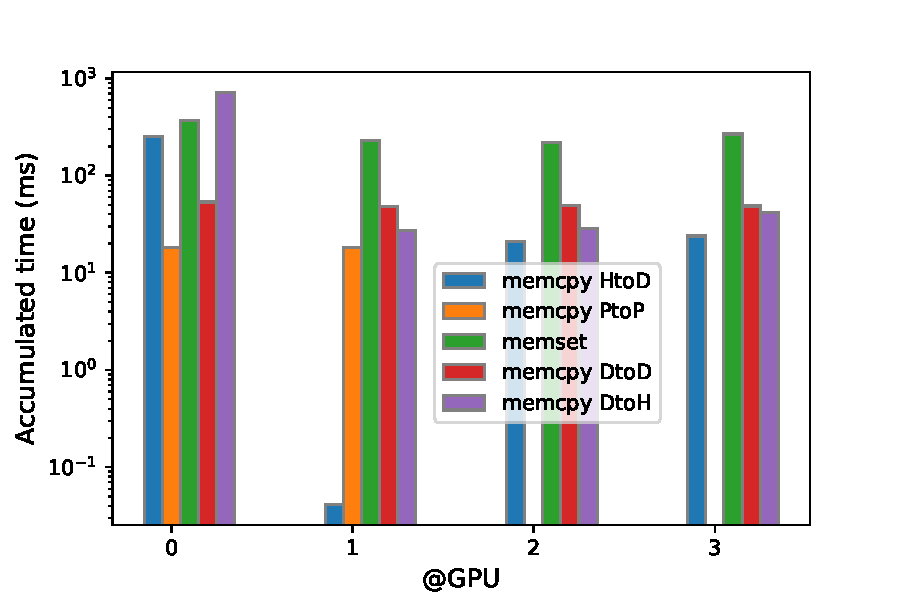
\includegraphics[width=\linewidth]{fig/bert/mem_4gpus.pdf}
      \caption{4 GPUs}
    \end{subfigure}
    \caption{Aggregated runtime of the built-in memory management operations}
\label{fig:bert:mem_mgnt}
\end{figure}


Since the memory management operations is likely to be the main factor of the poor speed up factor. Digging into their sub-group operations especially the built-in memory allocation and transfer function could bring us closer to the root cause of the communication overhead. Figure~\ref{fig:bert:mem_mgnt} demonstrates the aggregated run-time in each built-in operations. There is an asymmetric behaviour in the memory transfer of host-to-device and device-to-host where the second GPU barely see host-to-device operation for both cases. Moreover, the first GPU tends to volunteer to do this task. Device-to-host operation is more balance with a little asymmetry in the first GPU that they are significantly does consume more run-time by one order of magnitude.


\subsection{GPT-2}

\subsubsection{Configurations}

The configurations for GPT-2 model are as follows:

\begin{itemize}
    \item Batch size: 4
    \item GPU: 1, 2 and 4
    \item Model name: DistilGPT2 (the smallest version of GPT2)
    \item Dataset: Yelp Dataset (Text Classification)
    \item Epoch: 1
\end{itemize}

\subsubsection{Results}

Similar to BERT model, the top 10 most longest running interfaces in GPT-2 does have the same problem with communication overhead. Considering the Figure~\ref{fig:gpt2:tg}, The collective communication operators even appears when we train on a couple of GPUs and it getting worse when the number of GPUs reaching to four.

\begin{figure}[htbp]
    \centering
    \begin{subfigure}{.5\textwidth}
        \centering
        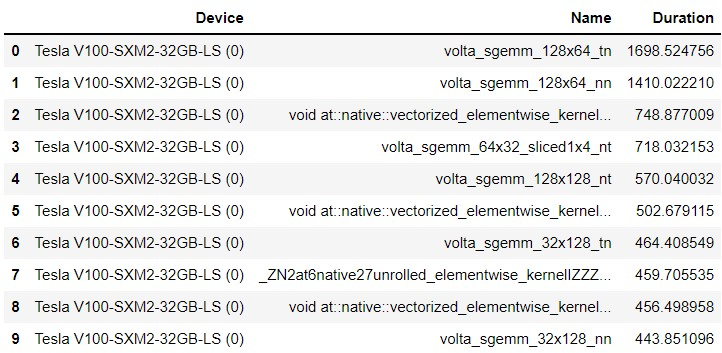
\includegraphics[width=\linewidth]{fig/gpt2/gpt_t1.jpg}
        \caption{1 GPUs}
        \label{fig:gpt2:timegroup}
    \end{subfigure}%
    \begin{subfigure}{.5\textwidth}
        \centering
        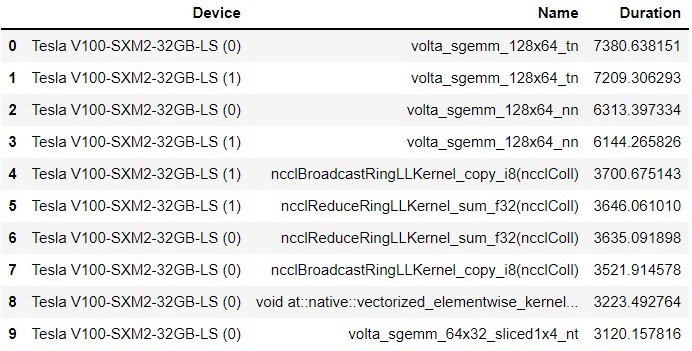
\includegraphics[width=\linewidth]{fig/gpt2/gpt_t2.jpg}
        \caption{2 GPUs}
        \label{fig:gpt2:timegroup_frac}
    \end{subfigure}
    \begin{subfigure}{.6\textwidth}
        \centering
        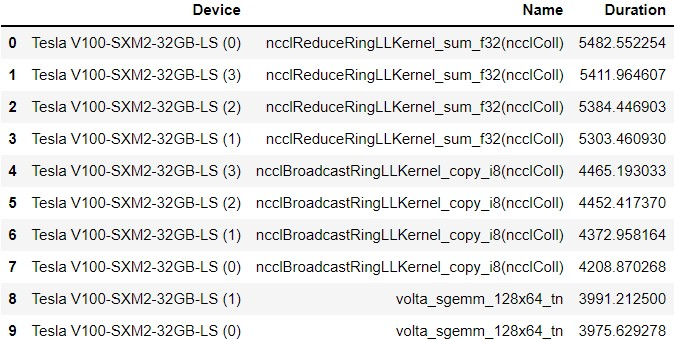
\includegraphics[width=\linewidth]{fig/gpt2/gpt_t4.jpg}
        \caption{4 GPUs}
        \label{fig:gpt2:timegroup_frac}
    \end{subfigure}    
    \caption{Top 10 longest running interfaces}
\label{fig:gpt2:tg}
\end{figure}

% For The big picture of the problem, It is like the results of the BERT model from visualizing the aggregated running time of each operation group as in Figure~\ref{fig:gpt2:group_runtime}
The trivial observations is illustrated in Figure~\ref{fig:gpt2:group_runtime}, it does have the same problem of data transfer where running on GPUs does spending more than one third of their time. Regarding to the Figure~\ref{fig:gpt2:mem}, the asymmetric in the host-to-device operation among running devices is more severe. The rest of them barely do host-to-device task. Surprisingly, memset operation is also unbalanced in four GPUs running which is not similar to a two GPUs and all benchmark in BERT.

\begin{figure}[htbp]
    \centering
    \begin{subfigure}{.5\textwidth}
        \centering
        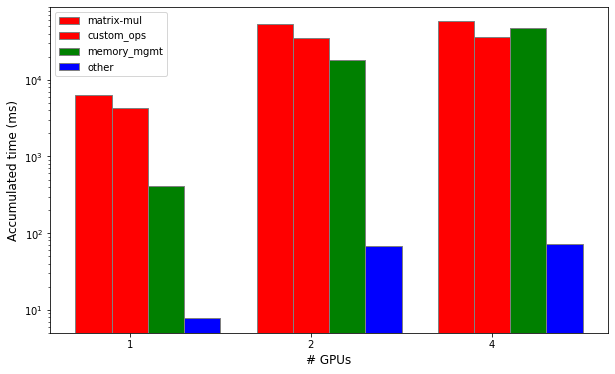
\includegraphics[width=\linewidth]{fig/gpt2/timegroup.png}
        \caption{Real spending time}
        \label{fig:gpt2:timegroup}
    \end{subfigure}%
    \begin{subfigure}{.5\textwidth}
        \centering
        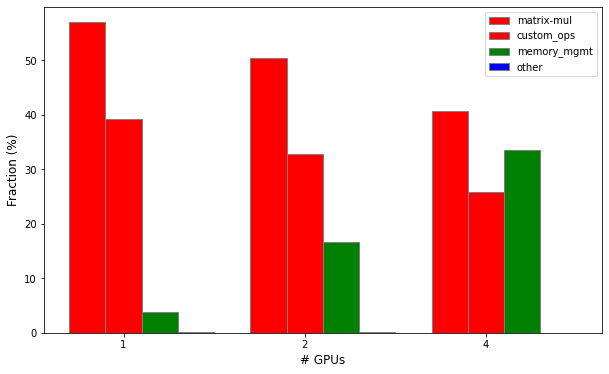
\includegraphics[width=\linewidth]{fig/gpt2/timegroup_frac.png}
        \caption{Fraction of time}
        \label{fig:gpt2:timegroup_frac}
    \end{subfigure}
    \caption{Spending time of multiple group of operations}
\label{fig:gpt2:group_runtime}
\end{figure}

\begin{figure}[htbp]
    \centering
    \begin{subfigure}{.5\textwidth}
      \centering
      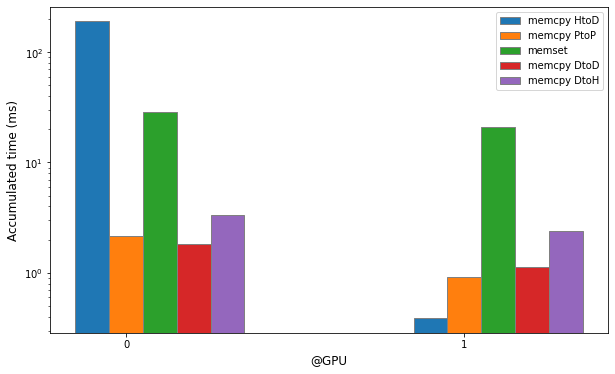
\includegraphics[width=\linewidth]{fig/gpt2/men_2gpu.png}
      \caption{2 GPUs}
      \label{fig:sub1}
    \end{subfigure}%
    \begin{subfigure}{.5\textwidth}
      \centering
      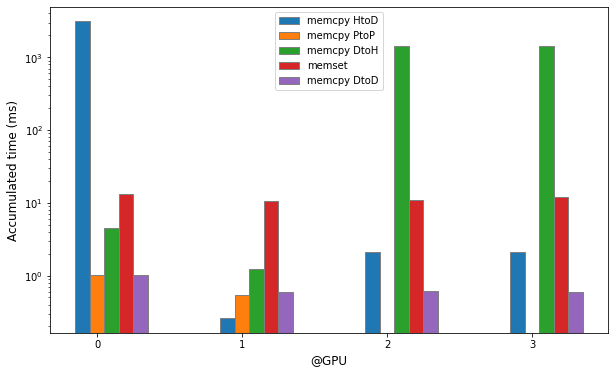
\includegraphics[width=\linewidth]{fig/gpt2/men_4gpu.png}
      \caption{4 GPUs}
      \label{fig:sub2}
    \end{subfigure}
    \caption{Aggregated runtime of the built-in memory management operations}
\label{fig:gpt2:mem}
\end{figure}

% \textcolor{red}{Discuss the result with figures}